\documentclass[aspectratio=169]{beamer}
\usepackage{csquotes}
\usepackage{booktabs}
%
% Choose how your presentation looks.
%
% For more themes, color themes and font themes, see:
% http://deic.uab.es/~iblanes/beamer_gallery/index_by_theme.html
%
\mode<presentation>
{
  \usetheme{default}      % or try Darmstadt, Madrid, Warsaw, ...
  \usecolortheme{default} % or try albatross, beaver, crane, ...
  \usefonttheme{default}  % or try serif, structurebold, ...
  \setbeamertemplate{navigation symbols}{}
  \setbeamertemplate{caption}[numbered]
} 

\usepackage[english]{babel}
\usepackage[utf8]{inputenc}
\usepackage[T1]{fontenc}
\usepackage{graphicx}
\usepackage{booktabs}
\usepackage{minted}
\newcommand{\hip}{\textbf{\color{red}{hip}}}

\usepackage[binary-units]{siunitx}
\usepackage{hyperref}
\newcommand{\gbs}{\si[per-symbol = \text{~div~}]{\gibi\byte\per\second}}

\title[]{HIP demo: \\ Multi-GPU Jacobi solver}
%\author{You}
% \institute{Where You're From}
%\date{Date of Presentation}

\begin{document}

\begin{frame}
  \titlepage
\end{frame}

\begin{frame}{Jacobi solver}
\begin{itemize}
    \item Solve Poison equation.
    \item Fixed boundary condition.
    \item Average of direct neighbors.
\end{itemize}
\begin{figure}[hb!]
    \centering
    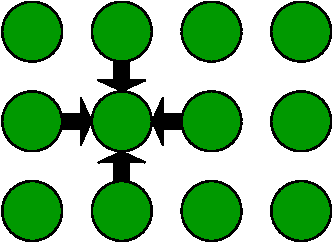
\includegraphics[scale=0.5]{figs/jacobi.pdf}
    % \caption{Caption}
    \label{fig:my_label}
\end{figure}
\end{frame}

% \begin{frame}[fragile]{Code, explanation}
\begin{frame}{The code}
\begin{itemize}
    \item Cuda code written by Nvidia.\footnote{\url{https://devblogs.nvidia.com/benchmarking-cuda-aware-mpi/}}
    \item 2d domain decomposition.
    \item MPI for communication between GPU's.
    \item Halo rows exchanged after each iteration.
\end{itemize}
\begin{figure}[hb!]
    \centering
    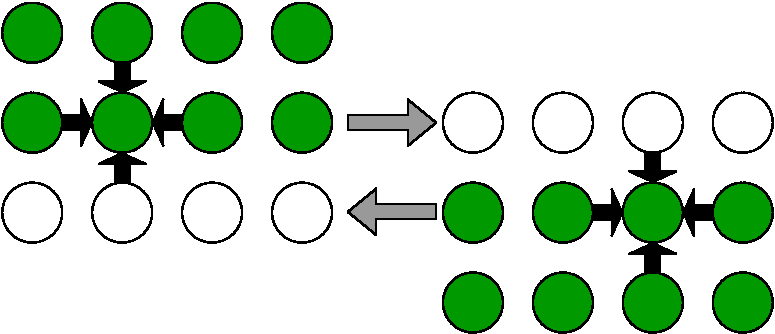
\includegraphics[scale=0.5]{figs/halo_sharing.pdf}
    % \caption{Caption}
    \label{fig:my_label}
\end{figure}

% \begin{minted}[
% frame=lines,
% framesep=3mm,
% escapeinside=||
% ]{c}
% Anew[j][i] = 0.25f * (A[j][i+1] + A[j-1][i] + A[j+1][i] + A[j][i-1]);
% \end{minted}

\end{frame}

\begin{frame}{Live demo}
\end{frame}

\begin{frame}{Some numbers}
% Please add the following required packages to your document preamble:
\begin{table}[]
\begin{tabular}{@{}lcc@{}}
\toprule
\multicolumn{1}{c}{}  & \# GPU's & GFLOPS / GPU \\ \midrule
TitanX                & 1        &     66.47    \\
MI50                  & 1        &     42.70    \\
MI50 same island      & 2        &     39.70    \\
MI50 different island & 2        &     27.60    \\
MI50 same island      & 4        &     38.44    \\ \bottomrule
\end{tabular}
\end{table}
\end{frame}

\begin{frame}{Conclusion}
\begin{itemize}
    \item The tools are straight forward to use.
    \item Can't blindly trust the tools.
    \item Understanding performance might require more in depth analysis.
\end{itemize}
\end{frame}

\end{document}
